\documentclass[spanish,a4paper,11pt,twoside]{report}

%%%%%%%%%%%%%%%%%%%%%%%%%%%%%%%%%%%%%%%%%%%%%%%%%%%%%%%%%%%%%%%%%%%%%%%%%%%%%%%
\usepackage[dvips]{graphicx}
\usepackage[dvips]{epsfig}
\usepackage[latin1]{inputenc}
\usepackage[spanish]{babel}
\usepackage{alltt}
\usepackage{templates/algorithm}
\usepackage{templates/algorithmic}
\usepackage{templates/multirow}

%%%%%%%%%%%%%%%%%%%%%%%%%%%%%%%%%%%%%%%%%%%%%%%%%%%%%%%%%%%%%%%%%%%%%%%%%%%%%%%

\newcommand{\SONY}{{\sc Sony}}
\newcommand{\MICROSOFT}{{\sc Microsoft}}
\newcommand{\GCC}{\textsf{\textsc{G}CC}}
\newcommand{\INTEL}{\textsf{\textsc{I}ntel}}

%%% Traducimos el pseudocodigo
\renewcommand{\algorithmicwhile}{\textbf{mientras}}
\renewcommand{\algorithmicend}{\textbf{fin}}
\renewcommand{\algorithmicdo}{\textbf{hacer}}
\renewcommand{\algorithmicif}{\textbf{si}}
\renewcommand{\algorithmicthen}{\textbf{entonces}}
\renewcommand{\algorithmicrepeat}{\textbf{repetir}}
\renewcommand{\algorithmicuntil}{\textbf{hasta que}}
\renewcommand{\algorithmicelse}{\textbf{en otro caso}}
\renewcommand{\algorithmicfor}{\textbf{para}}

%\newcommand{\RETURN}{\textbf{retornar} }
\newcommand{\RET}{\STATE \textbf{retornar} }
\newcommand{\TO}{\textbf{hasta} }
\newcommand{\AND}{\textbf{y} }
\newcommand{\OR}{\textbf{o} }

%%%%%%%%%%%%%%%%% Creamos un entorno para listar c�digo fuente %%%%%%%%%%%%%%%
\newenvironment{sourcecode}
{\begin{list}{}{\setlength{\leftmargin}{1em}}\item\scriptsize\bfseries}
{\end{list}}

\newenvironment{littlesourcecode}
{\begin{list}{}{\setlength{\leftmargin}{1em}}\item\tiny\bfseries}
{\end{list}}

\newenvironment{summary}
{\par\noindent\begin{center}\textbf{Abstract}\end{center}\begin{itshape}\par\noindent}
{\end{itshape}}

\newenvironment{keywords}
{\begin{list}{}{\setlength{\leftmargin}{1em}}\item[\hskip\labelsep \bfseries Keywords:]}
{\end{list}}

\newenvironment{palabrasClave}
{\begin{list}{}{\setlength{\leftmargin}{1em}}\item[\hskip\labelsep \bfseries Palabras clave:]}
{\end{list}}


%%%%%%%%%%%%%%%%%%%%%%%%%%%%%%%%%%%%%%%%%%%%%%%%%%%%%%%%%%%%%%%%%%%%%%%%%%%%%%%
% Format
%%%%%%%%%%%%%%%%%%%%%%%%%%%%%%%%%%%%%%%%%%%%%%%%%%%%%%%%%%%%%%%%%%%%%%%%%%%%%%%

%%\topmargin -4 mm
%\topmargin -21 mm
%\headheight 10 mm
%\headsep 10 mm

%\textheight 229 mm
%\textheight 246 mm

%\oddsidemargin -5.4 mm
%\evensidemargin -5.4 mm
\oddsidemargin 5 mm
\evensidemargin 5 mm

%\oddsidemargin -3 mm
%\evensidemargin -3 mm

%\textwidth 17 cm
\textwidth 15 cm
%\columnsep 10 mm

\input{amssym.def}

%%%%%%%%%%%%%%%%%%%%%%%%%%%%%%%%%%%%%%%%%%%%%%%%%%%%%%%%%%%%%%%%%%%%%%%%%%%%%%%

\begin{document}

%%%%%%%%%%%%%%%%%%%%%%%%%%%%%%%%%%%%%%%%%%%%%%%%%%%%%%%%%%%%%%%%%%%%%%%%%%%%%%%
% First Page 
%%%%%%%%%%%%%%%%%%%%%%%%%%%%%%%%%%%%%%%%%%%%%%%%%%%%%%%%%%%%%%%%%%%%%%%%%%%%%%%

\pagestyle{empty}
\thispagestyle{empty}


\newcommand{\HRule}{\rule{\linewidth}{1mm}}
\setlength{\parindent}{0mm}
\setlength{\parskip}{0mm}
\vspace*{\stretch{1}}

\begin{center}

\includegraphics[width=0.2\textwidth]{images/logotipo-secundario-ULL}\\[0.25cm]
\end{center}

\HRule
\begin{center}
        {\Huge T�tulo del trabajo} \\[2.5mm] 
        {\Huge Subt�tulo} \\[2.5mm]
        {\Large Autor (o autores)} \\[5mm]
        {\Large \textit{Grupo ($1\mid2$) }} \\[5mm]


        {\em T�cnicas Experimentales. $1^{er}$ curso. $2^{do}$ semestre} \\[5mm]
        Lenguajes y Sistemas Inform�ticos \\[5mm]
        Facultad de Matem�ticas \\[5mm]
        
        Universidad de La Laguna \\
\end{center}
\HRule
\vspace*{\stretch{2}}
\begin{center}
  La Laguna, \today 
\end{center}

%%%%%%%%%%%%%%%%%%%%%%%%%%%%%%%%%%%%%%%%%%%%%%%%%%%%%%%%%%%%%%%%%%%%%%%%%%%%%%%

%%%%%%%%%%%%%%%%%%%%%%%%%%%%%%%%%%%%%%%%%%%%%%%%%%%%%%%%%%%%%%%%%%%%%%%%%%%%%%%
\newpage{\pagestyle{empty}\cleardoublepage}

\pagestyle{myheadings} %my head defined by markboth or markright
% No funciona bien \markboth sin "twoside" en \documentclass, pero al
% ponerlo se dan un mont�n de errores de underfull \vbox, con lo que no se
% ha puesto.
\markboth{Nombre del alumno}{T�tulo del trabajo}

%%%%%%%%%%%%%%%%%%%%%%%%%%%%%%%%%%%%%%%%%%%%%%%%%%%%%%%%%%%%%%%%%%%%%%%%%%%%%%%
%Numeracion en romanos
\renewcommand{\thepage}{\roman{page}}
\setcounter{page}{1}

%%%%%%%%%%%%%%%%%%%%%%%%%%%%%%%%%%%%%%%%%%%%%%%%%%%%%%%%%%%%%%%%%%%%%%%%%%%%%%%

\tableofcontents

%%%%%%%%%%%%%%%%%%%%%%%%%%%%%%%%%%%%%%%%%%%%%%%%%%%%%%%%%%%%%%%%%%%%%%%%%%%%%%%
\newpage{\pagestyle{empty}\cleardoublepage}

\listoffigures

%%%%%%%%%%%%%%%%%%%%%%%%%%%%%%%%%%%%%%%%%%%%%%%%%%%%%%%%%%%%%%%%%%%%%%%%%%%%%%%
\newpage{\pagestyle{empty}\cleardoublepage}

\listoftables

%%%%%%%%%%%%%%%%%%%%%%%%%%%%%%%%%%%%%%%%%%%%%%%%%%%%%%%%%%%%%%%%%%%%%%%%%%%%%%%
\newpage{\pagestyle{empty}\cleardoublepage}

%%%%%%%%%%%%%%%%%%%%%%%%%%%%%%%%%%%%%%%%%%%%%%%%%%%%%%%%%%%%%%%%%%%%%%%%%%%%%%%
%Numeracion a partir del capitulo I
\renewcommand{\thepage}{\arabic{page}}
\setcounter{page}{1}

\setlength{\parindent}{5mm}

%%%%%%%%%%%%%%%%%%%%%%%%%%%%%%%%%%%%%%%%%%%%%%%%%%%%%%%%%%%%%%%%%%%%%%%%%%%%%%%
\chapter{Motivaci�n y objetivos}
\label{chapter:obj}

%%%%%%%%%%%%%%%%%%%%%%%%%%%%%%%%%%%%%%%%%%%%%%%%%%%%%%%%%%%%%%%%%%%%%%%%%%%%%
% Chapter 1: Motivaci�n y Objetivos 
%%%%%%%%%%%%%%%%%%%%%%%%%%%%%%%%%%%%%%%%%%%%%%%%%%%%%%%%%%%%%%%%%%%%%%%%%%%%%%%

Los objetivos le dan al lector las razones por las que se realiz� el
proyecto o trabajo de investigaci�n.

%---------------------------------------------------------------------------------
\section{Secci�n Uno}
\label{1:sec:1}
  Primer p�rrafo de la primera secci�n.
  Si simplemente se desea escribir texto normal en LaTeX,
  sin complicadas f�rmulas matem�ticas o efectos especiales
  como cambios de fuente, entonces simplemente tiene que escribir
  es espa�ol normalmente. \par
  Si desea cambiar el p�rrafo ha de dejar una l�nea en blanco o bien
  utilizar el comando \par
  No es necesario preocuparse de la sangr�a de los p�rrafos:
  todos los p�rrafos se sangrar�n autom�ticamente con la excepci�n
  del primer p�rrafo de una secci�n.
  
  Se ha de distinguir entre la comilla simple 'izquierda'
  y la comilla simple 'derecha' cuando se escribe en el ordenador.
  
  En el caso de que se quieran utilizar comillas dobles se han de 
  escribir dos caracteres 'comilla simple' seguidos, esto es, 
  ''comillas dobles''.
  
  Tambi�n se ha de tener cuidado con los guiones: se utiliza un �nico
  gui�n para la separaci�n de s�labas, mientras que se utilizan
  tres guiones seguidos para producir un gui�n de los que se usan 
  como signo de puntuaci�n ---como en esta oraci�n.
  


%---------------------------------------------------------------------------------
\section{Secci�n Dos}
\label{1:sec:2}
  Primer p�rrafo de la segunda secci�n.

\begin{itemize}
  \item Item 1
  \item Item 2
  \item Item 3
\end{itemize}



%%%%%%%%%%%%%%%%%%%%%%%%%%%%%%%%%%%%%%%%%%%%%%%%%%%%%%%%%%%%%%%%%%%%%%%%%%%%%%%
\chapter{Fundamentos te�ricos}
\label{chapter:teo}

%%%%%%%%%%%%%%%%%%%%%%%%%%%%%%%%%%%%%%%%%%%%%%%%%%%%%%%%%%%%%%%%%%%%%%%%%%%%%%%
% Chapter 2: Fundamentos Te�ricos 
%%%%%%%%%%%%%%%%%%%%%%%%%%%%%%%%%%%%%%%%%%%%%%%%%%%%%%%%%%%%%%%%%%%%%%%%%%%%%%%

%++++++++++++++++++++++++++++++++++++++++++++++++++++++++++++++++++++++++++++++

En este cap�tulo se han de presentar los antecedentes te�ricos y pr�cticos que
apoyan el tema objeto de la investigaci�n.

%++++++++++++++++++++++++++++++++++++++++++++++++++++++++++++++++++++++++++++++

\section{Primer apartado del segundo cap�tulo}
\label{2:sec:1}
  Primer p�rrafo de la primera secci�n.

En \LaTeX{}~\cite{Lamport:LDP94} es sencillo escribir expresiones
matem�ticas como $a=\sum_{i=1}^{10} {x_i}^{3}$
y deben ser escritas entre dos s�mbolos \$.
Los super�ndices se obtienen con el s�mbolo \^{}, y
los sub�ndices con el s�mbolo \_.
Por ejemplo: $x^2 \times y^{\alpha + \beta}$.
Tambi�n se pueden escribir f�rmulas centradas:
\[h^2=a^2 + b^2 \]

\section{Segundo apartado del segundo cap�tulo}
\label{2:sec:2}
  Primer p�rrafo de la segunda secci�n.



%%%%%%%%%%%%%%%%%%%%%%%%%%%%%%%%%%%%%%%%%%%%%%%%%%%%%%%%%%%%%%%%%%%%%%%%%%%%%%%
\chapter{Procedimiento experimental}
\label{chapter:exp}

%%%%%%%%%%%%%%%%%%%%%%%%%%%%%%%%%%%%%%%%%%%%%%%%%%%%%%%%%%%%%%%%%%%%%%%%%%%%%%%
% Cap�tulo 3: Procedimiento experimental 
%%%%%%%%%%%%%%%%%%%%%%%%%%%%%%%%%%%%%%%%%%%%%%%%%%%%%%%%%%%%%%%%%%%%%%%%%%%%%%%

%++++++++++++++++++++++++++++++++++++++++++++++++++++++++++++++++++++++++++++++
\section{Descripci�n de los experimentos}
\label{3:sec:1}
\setlength{\parskip}{2mm}

Para llevar a cabo el c�lculo de las ra�ces de la funci�n objeto de estudio,
se ha realizado la implementaci�n de un algoritmo recursivo basado en el m�todo
de Newton-Raphson (ver ap�ndice A). Ejecutando en repetidas ocasiones el fichero
resultante y utilizando distintos valores como par�metros iniciales del m�todo,
ha sido posible observar los efectos producidos por la variabilidad de �stos 
sobre la soluci�n final generada por el algoritmo.

Por otra parte, con el fin de cumplir los objetivos espec�ficos de esta investigaci�n
(ver cap�tulo 1), hemos recurrido a la elaboraci�n de tres programas Python: el primero 
de ellos (ap�ndice B1) est� destinado a efectuar un recuento de las iteraciones
requeridas para el c�lculo de una ra�z en funci�n del error absoluto del valor
proporcionado al m�todo como estimaci�n inicial, almacenando las cantidades obtenidas
en un fichero para su posterior lectura; el segundo (ap�ndice B2) posibilita la elaboraci�n 
de una gr�fica ilustrativa tomando como base la informaci�n contenida en el fichero generado 
con anterioridad, y el tercero (ap�ndice B3) cumple la funci�n de generar una representaci�n 
gr�fica del tiempo total de CPU empleado en la ejecuci�n del algoritmo, frente a la cantidad 
de iteraciones recursivas efectuadas por el mismo.

%++++++++++++++++++++++++++++++++++++++++++++++++++++++++++++++++++++++++++++++
\section{Descripci�n del material}
\label{3:sec:2}
\setlength{\parskip}{2mm}

Como soporte f�sico requerido para la puesta en pr�ctica de los experimentos,
ha sido utilizada una computadora con las especificaciones de hardware que se 
detallan a continuaci�n:

\begin{itemize}
    \item
      \textbf{Tipo de CPU:} Pentium(R) Dual-Core CPU, GenuineIntel, T4500.
    \item
      \textbf{Velocidad de la CPU:} 1200 Hz.
    \item
      \textbf{Tama�o del cach�:} 1024 KB.
    \item
      \textbf{Memoria RAM:} 8 GB.
\end{itemize}

En lo referente a las caracter�sticas y versiones del software empleado, cabe 
se�alar la siguente informaci�n:

\begin{itemize}
    \item
      \textbf{Versi�n de Python:} 2.7.3.
    \item
      \textbf{Compilador Python:} GCC 4.7.2.
    \item
      \textbf{Sistema operativo:} Linux-3.5.0-17-gen�rico con Ubuntu-12.10-quantal.
    \item
      \textbf{Fecha de creaci�n de la versi�n de Python:} Sep 26 2012 21:53:58.
\end{itemize}

%++++++++++++++++++++++++++++++++++++++++++++++++++++++++++++++++++++++++++++++
\section{Resultados obtenidos}
\label{3:sec:3}
\setlength{\parskip}{2mm}

La ejecuci�n del algoritmo implementado (ver ap�ndice A), basado en el m�todo de 
Newton-Raphson, para el c�lculo de las ra�ces de la funci�n $f(x) = cos (\pi x)$
ha proporcionado como resultado la siguiente tabla ejemplificativa de ra�ces, 
tomando como punto de partida los valores supuestos que en ella se especifican:

%--------------------------------------------------------------------------
\begin{table}
\end{table}
\begin{table}[H]
\begin{center}
\begin{tabular}{|c|c|c|c|c|}

   \hline
   \textbf{INICIO}  & \textbf{TOLERANCIA}  & \textbf{COTA ITERAC.} & \textbf{ITERAC. REALES} & \textbf{RESULTADO}  \\ \hline
   -7.08            & $10^{-7}$            & 100                   & 3                       & -8.5                \\ \hline
   -7.1             & $10^{-7}$            & 100                   & 4                       & -9.5                \\ \hline
   -7.2             & $10^{-7}$            & 100                   & 3                       & -7.5                \\ \hline
   -5.8             & $10^{-5}$            & 50                    & 2                       & -5.49999728877      \\ \hline
   -5.8             & $10^{-6}$            & 50                    & 3                       & -5.5                \\ \hline
   -0.23            & $10^{-7}$            & 30                    & 3                       & -0.5                \\ \hline
   -0.23            & $10^{-9}$            & 30                    & 3                       & -0.5                \\ \hline
   1.24             & $10^{-6}$            & 20                    & 2                       & 1.50000001507       \\ \hline
   1.24             & $10^{-8}$            & 20                    & 3                       & 1.5                 \\ \hline
   2.17             & $10^{-12}$           & 10                    & 4                       & 2.5                 \\ \hline
   3.45             & $10^{-4}$            & 10                    & 1                       & 3.49999999976       \\ \hline
   3.45             & $10^{-10}$           & 10                    & 2                       & 3.5                 \\ \hline
   
\end{tabular}
\end{center}
\caption{Resultados experimentales del algoritmo de Newton-Raphson}
\label{nwtable}
\end{table}
%--------------------------------------------------------------------------


En lo referente al an�lisis de la evoluci�n en la cantidad de iteraciones para
distintos errores absolutos o m�rgenes de desviaci�n en la estimaci�n inicial
respecto a la ra�z buscada, los resultados obtenidos quedan reflejados a trav�s
del siguiente gr�fico, basado en la tabla que a seguidamente se presenta y 
correspondientes a un margen de tolerancia de $10^{-9}$:

\begin{figure}[!th]
\begin{center}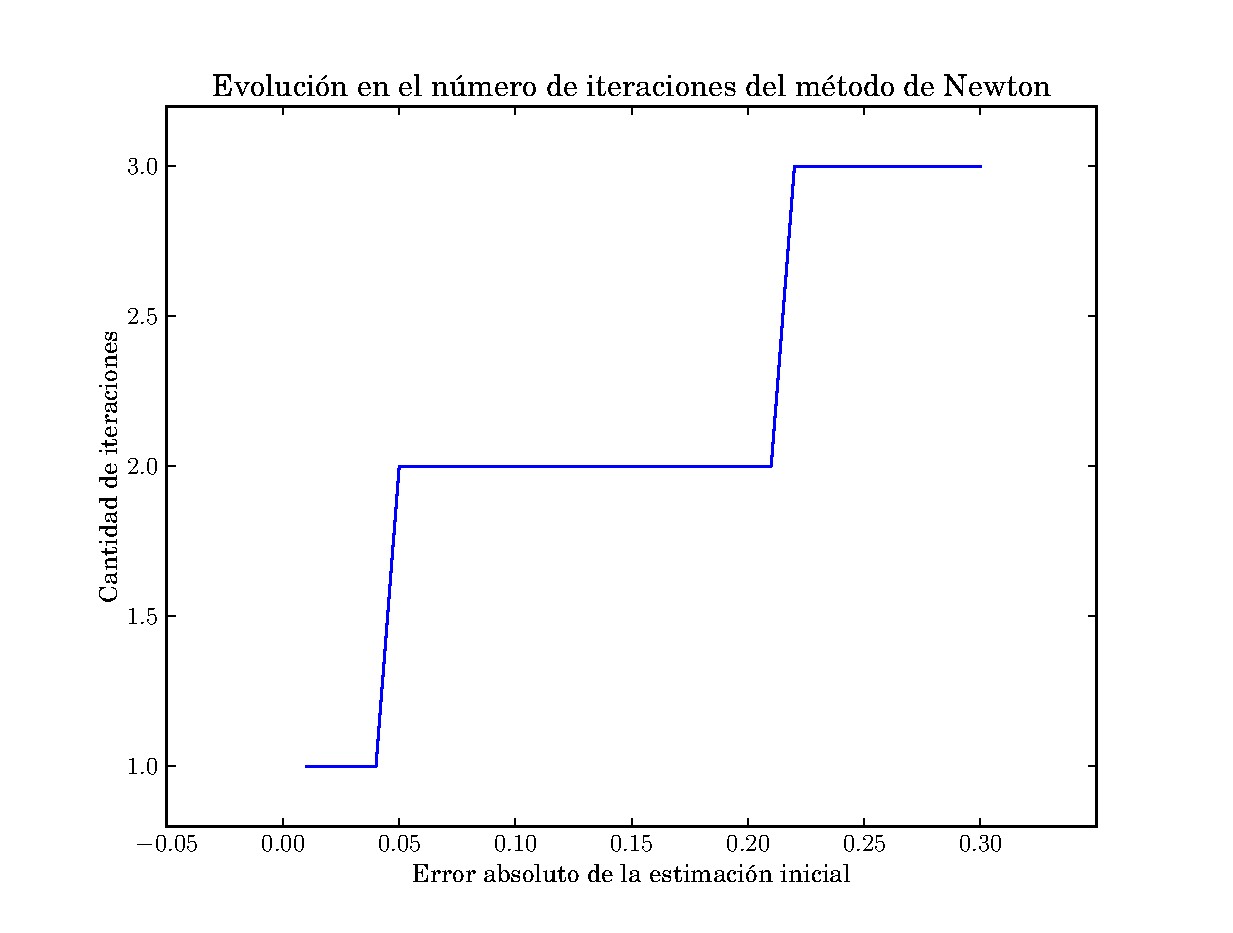
\includegraphics[height=11cm, width=14cm]{images/iterevol.eps}
\caption{An�lisis de la tendencia al incremento en las iteraciones.}
\label{iter}
\end{center}
\end{figure}

%--------------------------------------------------------------------------
\begin{table}
\end{table}
\begin{table}[H]
\begin{center}
\begin{tabular}{|c|c|c|}

   \hline
   \textbf{VALOR INICIAL}  & \textbf{ERROR ABSOLUTO}  & \textbf{ITERACIONES} \\ \hline
   Desde 0.2 hasta 0.28    & $e \in [0.22, 0.3]$      & 3                    \\ \hline
   Desde 0.29 hasta 0.45   & $e \in [0.05, 0.21]$     & 2                    \\ \hline    
   Desde 0.46 hasta 0.49   & $e \in [0.01, 0.04]$     & 1                    \\ \hline
   
\end{tabular}
\end{center}
\caption{Iteraciones requeridas para determinar $x_{0} = 0.5$}
\label{itertable}
\end{table}
%--------------------------------------------------------------------------


Por �ltimo, y siguiendo el esquema anterior, la informaci�n relativa al tiempo 
de CPU empleado para distintas cantidades de iteraciones puede consultarse a 
trav�s del gr�fico que a continuaci�n se muestra, as� como a partir de su tabla 
correspondiente:

\begin{figure}[!th]
\begin{center}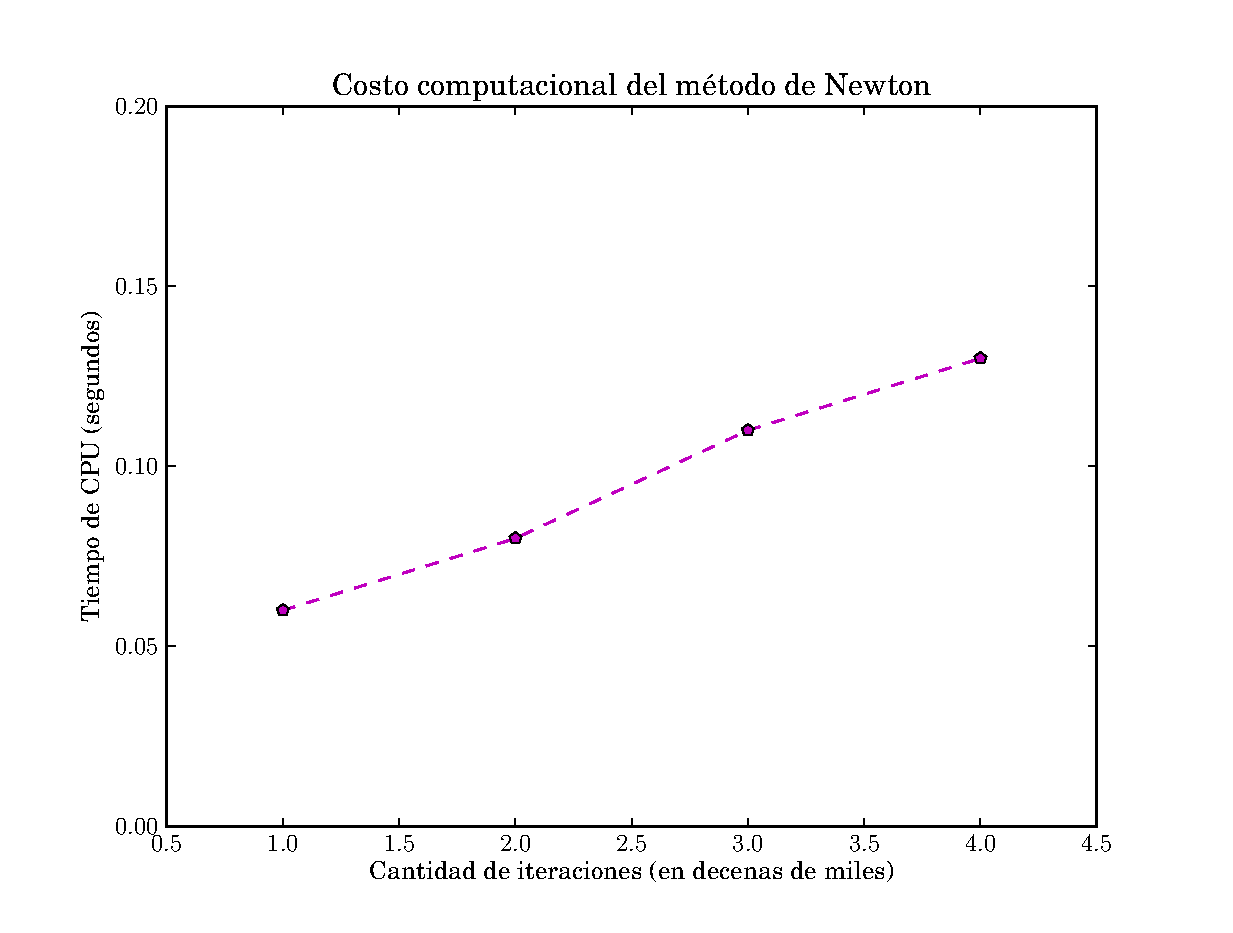
\includegraphics[height=11cm, width=14cm]{images/CPUtime.eps}
\caption{Avance del tiempo de CPU por cantidad de iteraciones.}
\label{cpu}
\end{center}
\end{figure}

%--------------------------------------------------------------------------
\begin{table}
\end{table}
\begin{table}[H]
\begin{center}
\begin{tabular}{|c|c|}

   \hline
   \textbf{ITERACIONES}  & \textbf{TIEMPO DE CPU} \\ \hline
   $10^{4}$              & 0.06 s                 \\ \hline
   $2 \cdot 10^{4}$      & 0.078 s                \\ \hline
   $3 \cdot 10^{4}$      & 0.11 s                 \\ \hline
   $4 \cdot 10^{4}$      & 0.13 s                 \\ \hline


\end{tabular}
\end{center}
\caption{Tiempo de CPU frente al volumen de iteraciones}
\label{cputable}
\end{table}
%--------------------------------------------------------------------------


%++++++++++++++++++++++++++++++++++++++++++++++++++++++++++++++++++++++++++++++
\section{An�lisis de los resultados}
\label{3:sec:4}
\setlength{\parskip}{2mm}

De acuerdo con informaci�n recogida en la tabla 3.1, es posible comentar diversos
aspectos relevantes. Por una parte, sus dos primeras filas reflejan un proceso de
ejecuci�n cuya iteraci�n inicial diverge respecto a la ra�z m�s cercana al valor
supuesto, debido a la proximidad del mismo a un extremo relativo de la funci�n, lo cual
origina una recta tangente de pendiente reducida cuyo punto de corte con los ejes se
encuentra notablemente alejado del valor de partida. Sin embargo, observamos que a 
partir de este momento la ejecuci�n recursiva se torna convergente, debido a que dicho
punto de corte constituye un valor supuesto pr�ximo a otra de las ra�ces de la funci�n
estudiada; en este sentido, podemos concluir que el m�todo de Newton-Raphson lograr�
la convergencia para la pr�ctica totalidad de los posibles valores iniciales, debido a
las infinitas ra�ces que la funci�n presenta y a su caracter�stica de periodicidad, si
bien la soluci�n devuelta por el m�todo podr�a no resultar la m�s pr�xima a la 
suposici�n inicial en caso de encontrarse �sta cercana a un extremo relativo de la
funci�n.

Por otra parte cabe destacar que, de modo general, la cantidad de iteraciones requerida
por este m�todo para la obtenci�n de una soluci�n v�lida resulta considerablemente reducida,
no superando las cuatro iteraciones a�n en el caso de seleccionar estrechos m�rgenes de 
tolerancia, del orden de $10^{-9}$; de acuerdo con ello, podemos afirmar que el m�todo
de Newton-Raphson presenta en este caso una elevada velocidad de convergencia. Debido a este
hecho, el valor fijado para la cota m�xima de iteraciones reviste escasa importancia, siendo
factible reducirlo hasta cantidades incluso inferiores a las diez iteraciones.

En lo referente al incremento en la cantidad de iteraciones en funci�n del aumento en el error
absoluto de la estimaci�n inicial respecto a la ra�z buscada, los datos recogidos en el gr�fico
3.1 y la tabla 3.2 corroboran lo ya observado con anterioridad: la r�pida convergencia del
algoritmo permite obtener un suave ascenso en el n�mero de ejecuciones recursivas, que tal y 
como ha sido expuesto, no llegan en ning�n caso a sobrepasar el margen de cuatro iteraciones.
De cualquier modo, la separaci�n constante de una unidad existente entre ra�ces imposibilita
el an�lisis del comportamiento del algoritmo para errores absolutos superiores a 0.3 en la 
estimaci�n inicial, a riesgo de comprometer la convergencia, producir una anulaci�n de la 
derivada u obtener ra�ces alejadas del entorno de partida.

Por �ltimo, la informaci�n relativa al costo computacional del algoritmo en t�rminos de tiempo
de CPU requerido para efectuar su ejecuci�n (v�ase figura 3.2 y tabla 3.3) nos permite corroborar
la elevada eficiencia de la implementaci�n recursiva del m�todo de Newton-Raphson, puesto que 
la reducida cantidad de iteraciones que requiere hace preciso reiterar decenas de miles de 
veces la invocaci�n al algoritmo hasta obtener valores significativos para los tiempos de uso de CPU.
Adem�s, observamos que la variabilidad en los par�metros iniciales tan s�lo afecta a la utilizaci�n
de recursos computacionales cuando su modificaci�n altera el volumen total de iteraciones requerido 
para la ejecuci�n del algoritmo. 



%%%%%%%%%%%%%%%%%%%%%%%%%%%%%%%%%%%%%%%%%%%%%%%%%%%%%%%%%%%%%%%%%%%%%%%%%%%%%%%
\chapter{Conclusiones}
\label{chapter:conclusiones}

%%%%%%%%%%%%%%%%%%%%%%%%%%%%%%%%%%%%%%%%%%%%%%%%%%%%%%%%%%%%%%%%%%%%%%%%%%%%%
% Chapter 4: Conclusiones y Trabajos Futuros 
%%%%%%%%%%%%%%%%%%%%%%%%%%%%%%%%%%%%%%%%%%%%%%%%%%%%%%%%%%%%%%%%%%%%%%%%%%%%%%%

bla, bla, bla, etc.


%%%%%%%%%%%%%%%%%%%%%%%%%%%%%%%%%%%%%%%%%%%%%%%%%%%%%%%%%%%%%%%%%%%%%%%%%%%%%%%

%%%%%%%%%%%%%%%%%%%%%%%%%%%%%%%%%%%%%%%%%%%%%%%%%%%%%%%%%%%%%%%%%%%%%%%%%%%%%%%
\newpage{\pagestyle{empty}\cleardoublepage}
\thispagestyle{empty}
\begin{appendix}

\chapter{T�tulo del Ap�ndice 1}
\label{appendix:1}

%%%%%%%%%%%%%%%%%%%%%%%%%%%%%%%%%%%%%%%%%%%%%%%%%%%%%%%%%%%%%%%%%%%%%%%%%%%%%%%%%%%%%%%
%           APÉNDICE 1
%%%%%%%%%%%%%%%%%%%%%%%%%%%%%%%%%%%%%%%%%%%%%%%%%%%%%%%%%%%%%%%%%%%%%%%%%%%%%%%%%%%%%%%

\begin{center}
\begin{footnotesize}

\begin{verbatim}
#######################################################################################
# Fichero newton.py
#######################################################################################
#
#  AUTORES: Alba Crespo Perez, Raquel Espino Mantas y Robbert Jozef Michiels
#   
#  FECHA: 5 de mayo de 2014
#
#  DESCRIPCION: Este codigo Python nos permite calcular las raices de la funcion
#  f(x) = cos (pi * x), mediante la aplicacion del metodo de Newton-Raphson. Como
#  parametros de inicio se solicita al usuario una estimacion de la raiz, el margen
#  de tolerancia permitido y una cota maxima de iteraciones.
#
#######################################################################################

#!encoding: UTF-8

from math import cos
from math import sin
PI = 3.141592653589793116

def f(x):
    return cos (PI * x)

def df(x):
    return - PI * sin (PI * x)

def newton (g, tol, nmax, it):
    if (it < nmax):
        if (df(g) != 0):
            g = g - (f(g)/df(g))
        else:
            return 1e7
        if (abs(f(g)) > tol):
            g = newton (g, tol, nmax, it)
            it = it + 1
        if (abs(f(g)) < tol):
            return g
    else:
        return 1e6

g = float(raw_input("\nProporcione una estimacion para iniciar el calculo: "))
tol = float(raw_input("Introduzca el margen de tolerancia: "))
nmax = int(raw_input("Indique la cantidad maxima de iteraciones: "))
it = 0
sol = newton (g, tol, nmax, it)
if (sol == 1e6):
    print "\n\tLo sentimos, no hemos localizado ninguna raiz \n\ttras alcanzar el maximo
            de iteraciones permitidas."
    print "\nIntentelo de nuevo proporcionando una mejor estimacion como inicio del método,\n
            o bien incrementando la cota de iteraciones.\n"
elif (sol == 1e7):
    print "\n\tHemos alcanzado una anulacion de la derivada durante la ejecucion, \n\tpor lo 
           que el metodo no es aplicable para los valores aportados.\n"
    print "Intentelo de nuevo modificando los parametros iniciales.\n"
else:
    print "\nRaiz encontrada para la funcion:", sol, "\n"

\end{verbatim}

\end{footnotesize}
\end{center}



\chapter{T�tulo del Ap�ndice 2}
\label{appendix:2}

\section{Recuento de iteraciones}
\label{Apendice2:label}

\begin{center}
\begin{footnotesize}

\begin{verbatim}
#######################################################################################
# Fichero countiter.py
#######################################################################################
#
#  AUTORES: Alba Crespo Perez, Raquel Espino Mantas y Robbert Jozef Michiels
#   
#  FECHA: 5 de mayo de 2014
#
#  DESCRIPCION: El codigo Python que a continuacion se presenta cumple la funcion
#  de determinar la cantidad de iteraciones requeridas para la deteccion de la raiz
#  x = 0.5, tomando como estimacion inicial a los distintos valores comprendidos en
#  el intervalo [0.2, 0.5), con una diferencia de una centesima entre dos valores 
#  consecutivos. Los resultados finales seran almacenados en un fichero.
#
#######################################################################################

#!encoding: UTF-8

from math import cos
from math import sin
PI = 3.141592653589793116

def f(x):
    return cos (PI * x)

def df(x):
    return - PI * sin (PI * x)

def newton (g, tol, nmax, it, name):
    if (it < nmax):
        if (df(g) != 0):
            g = g - (f(g)/df(g))
        else:
            return 1e7
        if (abs(f(g)) > tol):
            g = newton (g, tol, nmax, it, name)
            it = it + 1
        if (abs(f(g)) < tol):
            fich = open(name, "a")
            fich.write(str(it) + "\n")
            fich.close()
            return g
    else:
        return 1e6

tol = float(raw_input("\nIntroduzca el margen de tolerancia: "))
nmax = int(raw_input("Indique la cantidad maxima de iteraciones: "))
name = raw_input("Especifique un nombre para el fichero de salida: ")

for i in range (20, 50):
    x = i/100.0
    sol = newton (x, tol, nmax, 0, name)
    if (sol != 1e6) and (sol != 1e7):
        fich = open(name, "a")
        fich.write (str(x) + "\n")
        fich.close()

print "\nOperacion realizada con exito.\n"

\end{verbatim}

\end{footnotesize}
\end{center}

\section{Representacion grafica de la evolucion de las iteraciones}
\label{Apendice2:label2}

\begin{center}
\begin{footnotesize}

\begin{verbatim}
#######################################################################################
# Fichero graphiter.py
#######################################################################################
#
#  AUTORES: Alba Crespo Perez, Raquel Espino Mantas y Robbert Jozef Michiels
#   
#  FECHA: 5 de mayo de 2014
#
#  DESCRIPCION: A partir de la lectura e interpretacion de la informacion contenida
#  en el fichero generado por el programa anterior, este codigo nos permite elaborar
#  una representacion grafica de los datos experimentales obtenidos para asi facilitar 
#  su comprension y visualizacion. 
#
#######################################################################################

#!encoding: UTF-8

import matplotlib.pyplot as pl
pl.rc('text', usetex=True)
pl.rc('font', family='Bookman')

name = raw_input("Introduzca el nombre del fichero para lectura: ")
f = open(name, "r")

flag = 0
X = []
Y = []

while (True):
    l = f.readline().rstrip()
    if (l == ""):
        break
    elif (l != "0") and (l != "1"):
        Y = Y + [flag-1]
        flag = 0
    else:
        flag += 1

f.close()

for i in range (20, 50):
    x0 = i/100.0
    dif = 0.5 - x0
    X = X + [dif]

pl.plot(X,Y,"b")
pl.title(r'Evolucion en el numero de iteraciones del metodo de Newton') 
pl.xlabel(r'Error absoluto de la estimacion inicial')
pl.ylabel('Cantidad de iteraciones')

pl.xlim(-0.05, 0.35)
pl.ylim(0.8, 3.2)

pl.savefig("iterevol.eps", dpi=72)
pl.show()

\end{verbatim}


\end{footnotesize}
\end{center}


\end{appendix}

%%%%%%%%%%%%%%%%%%%%%%%%%%%%%%%%%%%%%%%%%%%%%%%%%%%%%%%%%%%%%%%%%%%%%%%%%%%%%%%
\addcontentsline{toc}{chapter}{Bibliograf�a}
\bibliographystyle{plain}


\bibliography{bib/references}
\nocite{*}

%%%%%%%%%%%%%%%%%%%%%%%%%%%%%%%%%%%%%%%%%%%%%%%%%%%%%%%%%%%%%%%%%%%%%%%%%%%%%%%

\end{document}
